\documentclass[1p]{elsarticle_modified}
%\bibliographystyle{elsarticle-num}

%\usepackage[colorlinks]{hyperref}
%\usepackage{abbrmath_seonhwa} %\Abb, \Ascr, \Acal ,\Abf, \Afrak
\usepackage{amsfonts}
\usepackage{amssymb}
\usepackage{amsmath}
\usepackage{amsthm}
\usepackage{scalefnt}
\usepackage{amsbsy}
\usepackage{kotex}
\usepackage{caption}
\usepackage{subfig}
\usepackage{color}
\usepackage{graphicx}
\usepackage{xcolor} %% white, black, red, green, blue, cyan, magenta, yellow
\usepackage{float}
\usepackage{setspace}
\usepackage{hyperref}

\usepackage{tikz}
\usetikzlibrary{arrows}

\usepackage{multirow}
\usepackage{array} % fixed length table
\usepackage{hhline}

%%%%%%%%%%%%%%%%%%%%%
\makeatletter
\renewcommand*\env@matrix[1][\arraystretch]{%
	\edef\arraystretch{#1}%
	\hskip -\arraycolsep
	\let\@ifnextchar\new@ifnextchar
	\array{*\c@MaxMatrixCols c}}
\makeatother %https://tex.stackexchange.com/questions/14071/how-can-i-increase-the-line-spacing-in-a-matrix
%%%%%%%%%%%%%%%

\usepackage[normalem]{ulem}

\newcommand{\msout}[1]{\ifmmode\text{\sout{\ensuremath{#1}}}\else\sout{#1}\fi}
%SOURCE: \msout is \stkout macro in https://tex.stackexchange.com/questions/20609/strikeout-in-math-mode

\newcommand{\cancel}[1]{
	\ifmmode
	{\color{red}\msout{#1}}
	\else
	{\color{red}\sout{#1}}
	\fi
}

\newcommand{\add}[1]{
	{\color{blue}\uwave{#1}}
}

\newcommand{\replace}[2]{
	\ifmmode
	{\color{red}\msout{#1}}{\color{blue}\uwave{#2}}
	\else
	{\color{red}\sout{#1}}{\color{blue}\uwave{#2}}
	\fi
}

\newcommand{\Sol}{\mathcal{S}} %segment
\newcommand{\D}{D} %diagram
\newcommand{\A}{\mathcal{A}} %arc


%%%%%%%%%%%%%%%%%%%%%%%%%%%%%5 test

\def\sl{\operatorname{\textup{SL}}(2,\Cbb)}
\def\psl{\operatorname{\textup{PSL}}(2,\Cbb)}
\def\quan{\mkern 1mu \triangleright \mkern 1mu}

\theoremstyle{definition}
\newtheorem{thm}{Theorem}[section]
\newtheorem{prop}[thm]{Proposition}
\newtheorem{lem}[thm]{Lemma}
\newtheorem{ques}[thm]{Question}
\newtheorem{cor}[thm]{Corollary}
\newtheorem{defn}[thm]{Definition}
\newtheorem{exam}[thm]{Example}
\newtheorem{rmk}[thm]{Remark}
\newtheorem{alg}[thm]{Algorithm}

\newcommand{\I}{\sqrt{-1}}
\begin{document}

%\begin{frontmatter}
%
%\title{Boundary parabolic representations of knots up to 8 crossings}
%
%%% Group authors per affiliation:
%\author{Yunhi Cho} 
%\address{Department of Mathematics, University of Seoul, Seoul, Korea}
%\ead{yhcho@uos.ac.kr}
%
%
%\author{Seonhwa Kim} %\fnref{s_kim}}
%\address{Center for Geometry and Physics, Institute for Basic Science, Pohang, 37673, Korea}
%\ead{ryeona17@ibs.re.kr}
%
%\author{Hyuk Kim}
%\address{Department of Mathematical Sciences, Seoul National University, Seoul 08826, Korea}
%\ead{hyukkim@snu.ac.kr}
%
%\author{Seokbeom Yoon}
%\address{Department of Mathematical Sciences, Seoul National University, Seoul, 08826,  Korea}
%\ead{sbyoon15@snu.ac.kr}
%
%\begin{abstract}
%We find all boundary parabolic representation of knots up to 8 crossings.
%
%\end{abstract}
%\begin{keyword}
%    \MSC[2010] 57M25 
%\end{keyword}
%
%\end{frontmatter}

%\linenumbers
%\tableofcontents
%
\newcommand\colored[1]{\textcolor{white}{\rule[-0.35ex]{0.8em}{1.4ex}}\kern-0.8em\color{red} #1}%
%\newcommand\colored[1]{\textcolor{white}{ #1}\kern-2.17ex	\textcolor{white}{ #1}\kern-1.81ex	\textcolor{white}{ #1}\kern-2.15ex\color{red}#1	}

{\Large $\underline{12a_{1039}~(K12a_{1039})}$}

\setlength{\tabcolsep}{10pt}
\renewcommand{\arraystretch}{1.6}
\vspace{1cm}\begin{tabular}{m{100pt}>{\centering\arraybackslash}m{274pt}}
\multirow{5}{120pt}{
	\centering
	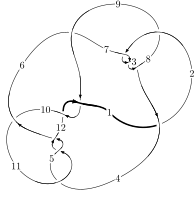
\includegraphics[width=112pt]{../../../GIT/diagram.site/Diagrams/png/1840_12a_1039.png}\\
\ \ \ A knot diagram\footnotemark}&
\allowdisplaybreaks
\textbf{Linearized knot diagam} \\
\cline{2-2}
 &
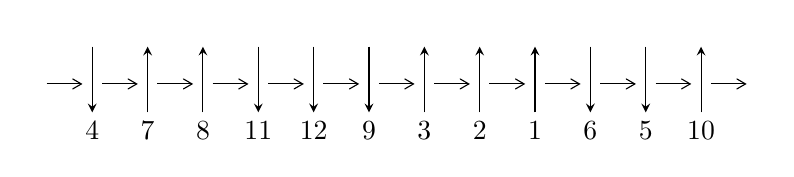
\begin{tikzpicture}[x=20pt, y=17pt]
	% nodes
	\node (C0) at (0, 0) {};
	\node (C1) at (1, 0) {};
	\node (C1U) at (1, +1) {};
	\node (C1D) at (1, -1) {4};

	\node (C2) at (2, 0) {};
	\node (C2U) at (2, +1) {};
	\node (C2D) at (2, -1) {7};

	\node (C3) at (3, 0) {};
	\node (C3U) at (3, +1) {};
	\node (C3D) at (3, -1) {8};

	\node (C4) at (4, 0) {};
	\node (C4U) at (4, +1) {};
	\node (C4D) at (4, -1) {11};

	\node (C5) at (5, 0) {};
	\node (C5U) at (5, +1) {};
	\node (C5D) at (5, -1) {12};

	\node (C6) at (6, 0) {};
	\node (C6U) at (6, +1) {};
	\node (C6D) at (6, -1) {9};

	\node (C7) at (7, 0) {};
	\node (C7U) at (7, +1) {};
	\node (C7D) at (7, -1) {3};

	\node (C8) at (8, 0) {};
	\node (C8U) at (8, +1) {};
	\node (C8D) at (8, -1) {2};

	\node (C9) at (9, 0) {};
	\node (C9U) at (9, +1) {};
	\node (C9D) at (9, -1) {1};

	\node (C10) at (10, 0) {};
	\node (C10U) at (10, +1) {};
	\node (C10D) at (10, -1) {6};

	\node (C11) at (11, 0) {};
	\node (C11U) at (11, +1) {};
	\node (C11D) at (11, -1) {5};

	\node (C12) at (12, 0) {};
	\node (C12U) at (12, +1) {};
	\node (C12D) at (12, -1) {10};
	\node (C13) at (13, 0) {};

	% arrows
	\draw[->,>={angle 60}]
	(C0) edge (C1) (C1) edge (C2) (C2) edge (C3) (C3) edge (C4) (C4) edge (C5) (C5) edge (C6) (C6) edge (C7) (C7) edge (C8) (C8) edge (C9) (C9) edge (C10) (C10) edge (C11) (C11) edge (C12) (C12) edge (C13) ;	\draw[->,>=stealth]
	(C1U) edge (C1D) (C2D) edge (C2U) (C3D) edge (C3U) (C4U) edge (C4D) (C5U) edge (C5D) (C6U) edge (C6D) (C7D) edge (C7U) (C8D) edge (C8U) (C9D) edge (C9U) (C10U) edge (C10D) (C11U) edge (C11D) (C12D) edge (C12U) ;
	\end{tikzpicture} \\
\hhline{~~} \\& 
\textbf{Solving Sequence} \\ \cline{2-2} 
 &
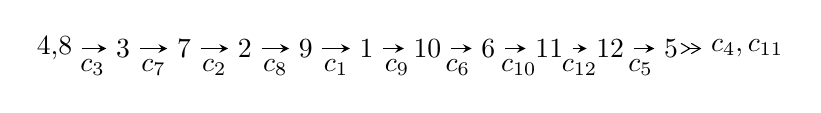
\begin{tikzpicture}[x=22pt, y=7pt]
	% node
	\node (A0) at (-1/8, 0) {4,8};
	\node (A1) at (1, 0) {3};
	\node (A2) at (2, 0) {7};
	\node (A3) at (3, 0) {2};
	\node (A4) at (4, 0) {9};
	\node (A5) at (5, 0) {1};
	\node (A6) at (6, 0) {10};
	\node (A7) at (7, 0) {6};
	\node (A8) at (8, 0) {11};
	\node (A9) at (9, 0) {12};
	\node (A10) at (10, 0) {5};
	\node (C1) at (1/2, -1) {$c_{3}$};
	\node (C2) at (3/2, -1) {$c_{7}$};
	\node (C3) at (5/2, -1) {$c_{2}$};
	\node (C4) at (7/2, -1) {$c_{8}$};
	\node (C5) at (9/2, -1) {$c_{1}$};
	\node (C6) at (11/2, -1) {$c_{9}$};
	\node (C7) at (13/2, -1) {$c_{6}$};
	\node (C8) at (15/2, -1) {$c_{10}$};
	\node (C9) at (17/2, -1) {$c_{12}$};
	\node (C10) at (19/2, -1) {$c_{5}$};
	\node (A11) at (45/4, 0) {$c_{4},c_{11}$};

	% edge
	\draw[->,>=stealth]	
	(A0) edge (A1) (A1) edge (A2) (A2) edge (A3) (A3) edge (A4) (A4) edge (A5) (A5) edge (A6) (A6) edge (A7) (A7) edge (A8) (A8) edge (A9) (A9) edge (A10) ;
	\draw[->>,>={angle 60}]	
	(A10) edge (A11);
\end{tikzpicture} \\ 

\end{tabular} \\

\footnotetext{
The image of knot diagram is generated by the software ``\textbf{Draw programme}" developed by Andrew Bartholomew(\url{http://www.layer8.co.uk/maths/draw/index.htm\#Running-draw}), where we modified some parts for our purpose(\url{https://github.com/CATsTAILs/LinksPainter}).
}\phantom \\ \newline 
\centering \textbf{Ideals for irreducible components\footnotemark of $X_{\text{par}}$} 
 
\begin{align*}
I^u_{1}&=\langle 
u^{68}- u^{67}+\cdots+3 u^2+1\rangle \\
\\
\end{align*}
\raggedright * 1 irreducible components of $\dim_{\mathbb{C}}=0$, with total 68 representations.\\
\footnotetext{All coefficients of polynomials are rational numbers. But the coefficients are sometimes approximated in decimal forms when there is not enough margin.}
\newpage
\renewcommand{\arraystretch}{1}
\centering \section*{I. $I^u_{1}= \langle u^{68}- u^{67}+\cdots+3 u^2+1 \rangle$}
\flushleft \textbf{(i) Arc colorings}\\
\begin{tabular}{m{7pt} m{180pt} m{7pt} m{180pt} }
\flushright $a_{4}=$&$\begin{pmatrix}1\\0\end{pmatrix}$ \\
\flushright $a_{8}=$&$\begin{pmatrix}0\\u\end{pmatrix}$ \\
\flushright $a_{3}=$&$\begin{pmatrix}1\\u^2\end{pmatrix}$ \\
\flushright $a_{7}=$&$\begin{pmatrix}- u\\- u^3+u\end{pmatrix}$ \\
\flushright $a_{2}=$&$\begin{pmatrix}- u^2+1\\- u^4+2 u^2\end{pmatrix}$ \\
\flushright $a_{9}=$&$\begin{pmatrix}u^5-2 u^3+u\\u^7-3 u^5+2 u^3+u\end{pmatrix}$ \\
\flushright $a_{1}=$&$\begin{pmatrix}- u^4+u^2+1\\- u^4+2 u^2\end{pmatrix}$ \\
\flushright $a_{10}=$&$\begin{pmatrix}u^{15}-6 u^{13}+12 u^{11}-6 u^9-6 u^7+4 u^5+2 u\\u^{15}-7 u^{13}+18 u^{11}-19 u^9+6 u^7-2 u^5+4 u^3+u\end{pmatrix}$ \\
\flushright $a_{6}=$&$\begin{pmatrix}- u^9+4 u^7-5 u^5+2 u^3- u\\- u^{11}+5 u^9-8 u^7+3 u^5+u^3+u\end{pmatrix}$ \\
\flushright $a_{11}=$&$\begin{pmatrix}u^{35}-16 u^{33}+\cdots-3 u^3+2 u\\u^{37}-17 u^{35}+\cdots+7 u^3+u\end{pmatrix}$ \\
\flushright $a_{12}=$&$\begin{pmatrix}- u^{26}+11 u^{24}+\cdots+3 u^2+1\\- u^{26}+12 u^{24}+\cdots+4 u^4+3 u^2\end{pmatrix}$ \\
\flushright $a_{5}=$&$\begin{pmatrix}- u^{63}+28 u^{61}+\cdots+22 u^5+12 u^3\\- u^{63}+29 u^{61}+\cdots+4 u^3+u\end{pmatrix}$\\&\end{tabular}
\flushleft \textbf{(ii) Obstruction class $= -1$}\\~\\
\flushleft \textbf{(iii) Cusp Shapes $= -4 u^{66}+124 u^{64}+\cdots+16 u-2$}\\~\\
\newpage\renewcommand{\arraystretch}{1}
\flushleft \textbf{(iv) u-Polynomials at the component}\newline \\
\begin{tabular}{m{50pt}|m{274pt}}
Crossings & \hspace{64pt}u-Polynomials at each crossing \\
\hline $$\begin{aligned}c_{1},c_{6}\end{aligned}$$&$\begin{aligned}
&u^{68}-11 u^{67}+\cdots-1692 u+113
\end{aligned}$\\
\hline $$\begin{aligned}c_{2},c_{3},c_{7}\end{aligned}$$&$\begin{aligned}
&u^{68}+u^{67}+\cdots+3 u^2+1
\end{aligned}$\\
\hline $$\begin{aligned}c_{4},c_{5},c_{11}\end{aligned}$$&$\begin{aligned}
&u^{68}- u^{67}+\cdots+3 u^2+1
\end{aligned}$\\
\hline $$\begin{aligned}c_{8}\end{aligned}$$&$\begin{aligned}
&u^{68}-3 u^{67}+\cdots+630 u-369
\end{aligned}$\\
\hline $$\begin{aligned}c_{9},c_{12}\end{aligned}$$&$\begin{aligned}
&u^{68}+11 u^{67}+\cdots+1692 u+113
\end{aligned}$\\
\hline $$\begin{aligned}c_{10}\end{aligned}$$&$\begin{aligned}
&u^{68}+3 u^{67}+\cdots-630 u-369
\end{aligned}$\\
\hline
\end{tabular}\\~\\
\newpage\renewcommand{\arraystretch}{1}
\flushleft \textbf{(v) Riley Polynomials at the component}\newline \\
\begin{tabular}{m{50pt}|m{274pt}}
Crossings & \hspace{64pt}Riley Polynomials at each crossing \\
\hline $$\begin{aligned}c_{1},c_{6},c_{9}\\c_{12}\end{aligned}$$&$\begin{aligned}
&y^{68}+49 y^{67}+\cdots+20218 y+12769
\end{aligned}$\\
\hline $$\begin{aligned}c_{2},c_{3},c_{4}\\c_{5},c_{7},c_{11}\end{aligned}$$&$\begin{aligned}
&y^{68}-63 y^{67}+\cdots+6 y+1
\end{aligned}$\\
\hline $$\begin{aligned}c_{8},c_{10}\end{aligned}$$&$\begin{aligned}
&y^{68}-19 y^{67}+\cdots-2666250 y+136161
\end{aligned}$\\
\hline
\end{tabular}\\~\\
\newpage\flushleft \textbf{(vi) Complex Volumes and Cusp Shapes}
$$\begin{array}{c|c|c}  
\text{Solutions to }I^u_{1}& \I (\text{vol} + \sqrt{-1}CS) & \text{Cusp shape}\\
 \hline 
\begin{aligned}
u &= \phantom{-}1.16639\phantom{ +0.000000I}\end{aligned}
 & -2.36439\phantom{ +0.000000I} & \phantom{-0.000000 } 0 \\ \hline\begin{aligned}
u &= \phantom{-}1.185360 + 0.209451 I\end{aligned}
 & -6.83305 - 1.72993 I & \phantom{-0.000000 } 0 \\ \hline\begin{aligned}
u &= \phantom{-}1.185360 - 0.209451 I\end{aligned}
 & -6.83305 + 1.72993 I & \phantom{-0.000000 } 0 \\ \hline\begin{aligned}
u &= -0.365893 + 0.690572 I\end{aligned}
 & -5.83372 - 10.83810 I & -3.95689 + 8.43769 I \\ \hline\begin{aligned}
u &= -0.365893 - 0.690572 I\end{aligned}
 & -5.83372 + 10.83810 I & -3.95689 - 8.43769 I \\ \hline\begin{aligned}
u &= -1.208360 + 0.195557 I\end{aligned}
 & -0.669905 - 1.153560 I & \phantom{-0.000000 } 0 \\ \hline\begin{aligned}
u &= -1.208360 - 0.195557 I\end{aligned}
 & -0.669905 + 1.153560 I & \phantom{-0.000000 } 0 \\ \hline\begin{aligned}
u &= \phantom{-}0.366622 + 0.678680 I\end{aligned}
 & \phantom{-0.000000 -}7.42138 I & \phantom{-0.000000 } 0. - 8.76802 I \\ \hline\begin{aligned}
u &= \phantom{-}0.366622 - 0.678680 I\end{aligned}
 & \phantom{-0.000000 } -7.42138 I & \phantom{-0.000000 -}0. + 8.76802 I \\ \hline\begin{aligned}
u &= -0.411460 + 0.633737 I\end{aligned}
 & \phantom{-}0.45656 - 5.12674 I & \phantom{-}0.57871 + 7.03241 I \\ \hline\begin{aligned}
u &= -0.411460 - 0.633737 I\end{aligned}
 & \phantom{-}0.45656 + 5.12674 I & \phantom{-}0.57871 - 7.03241 I \\ \hline\begin{aligned}
u &= -0.353617 + 0.662232 I\end{aligned}
 & -0.67977 - 3.43697 I & -1.83810 + 2.79608 I \\ \hline\begin{aligned}
u &= -0.353617 - 0.662232 I\end{aligned}
 & -0.67977 + 3.43697 I & -1.83810 - 2.79608 I \\ \hline\begin{aligned}
u &= \phantom{-}1.231400 + 0.212602 I\end{aligned}
 & -0.45656 + 5.12674 I & \phantom{-0.000000 } 0 \\ \hline\begin{aligned}
u &= \phantom{-}1.231400 - 0.212602 I\end{aligned}
 & -0.45656 - 5.12674 I & \phantom{-0.000000 } 0 \\ \hline\begin{aligned}
u &= \phantom{-}0.330337 + 0.672943 I\end{aligned}
 & -7.00321 + 0.97426 I & -5.71997 - 2.85709 I \\ \hline\begin{aligned}
u &= \phantom{-}0.330337 - 0.672943 I\end{aligned}
 & -7.00321 - 0.97426 I & -5.71997 + 2.85709 I \\ \hline\begin{aligned}
u &= -0.548441 + 0.510750 I\end{aligned}
 & -5.09005 + 6.77785 I & -2.21904 - 2.56386 I \\ \hline\begin{aligned}
u &= -0.548441 - 0.510750 I\end{aligned}
 & -5.09005 - 6.77785 I & -2.21904 + 2.56386 I \\ \hline\begin{aligned}
u &= -1.231440 + 0.231517 I\end{aligned}
 & -6.47567 - 8.30107 I & \phantom{-0.000000 } 0 \\ \hline\begin{aligned}
u &= -1.231440 - 0.231517 I\end{aligned}
 & -6.47567 + 8.30107 I & \phantom{-0.000000 } 0 \\ \hline\begin{aligned}
u &= \phantom{-}0.427107 + 0.604623 I\end{aligned}
 & \phantom{-}4.25225 + 1.96489 I & \phantom{-}6.41876 - 3.80214 I \\ \hline\begin{aligned}
u &= \phantom{-}0.427107 - 0.604623 I\end{aligned}
 & \phantom{-}4.25225 - 1.96489 I & \phantom{-}6.41876 + 3.80214 I \\ \hline\begin{aligned}
u &= -0.457025 + 0.579336 I\end{aligned}
 & \phantom{-}0.669905 + 1.153560 I & \phantom{-}1.403435 - 0.101236 I \\ \hline\begin{aligned}
u &= -0.457025 - 0.579336 I\end{aligned}
 & \phantom{-}0.669905 - 1.153560 I & \phantom{-}1.403435 + 0.101236 I \\ \hline\begin{aligned}
u &= \phantom{-}0.524039 + 0.507598 I\end{aligned}
 & \phantom{-}0.67977 - 3.43697 I & \phantom{-}1.83810 + 2.79608 I \\ \hline\begin{aligned}
u &= \phantom{-}0.524039 - 0.507598 I\end{aligned}
 & \phantom{-}0.67977 + 3.43697 I & \phantom{-}1.83810 - 2.79608 I \\ \hline\begin{aligned}
u &= -1.28430\phantom{ +0.000000I}\end{aligned}
 & \phantom{-}2.97683\phantom{ +0.000000I} & \phantom{-0.000000 } 0 \\ \hline\begin{aligned}
u &= \phantom{-}0.540694 + 0.417882 I\end{aligned}
 & -6.07300 + 2.79125 I & -3.29801 - 3.53193 I \\ \hline\begin{aligned}
u &= \phantom{-}0.540694 - 0.417882 I\end{aligned}
 & -6.07300 - 2.79125 I & -3.29801 + 3.53193 I\\
 \hline 
 \end{array}$$\newpage$$\begin{array}{c|c|c}  
\text{Solutions to }I^u_{1}& \I (\text{vol} + \sqrt{-1}CS) & \text{Cusp shape}\\
 \hline 
\begin{aligned}
u &= -0.484269 + 0.469339 I\end{aligned}
 & \phantom{-0.000000 } -0.351863 I & \phantom{-0.000000 -}0. + 3.89168 I \\ \hline\begin{aligned}
u &= -0.484269 - 0.469339 I\end{aligned}
 & \phantom{-0.000000 -}0.351863 I & \phantom{-0.000000 } 0. - 3.89168 I \\ \hline\begin{aligned}
u &= \phantom{-}0.026103 + 0.672070 I\end{aligned}
 & -10.31710 + 4.99618 I & -9.53537 - 3.59644 I \\ \hline\begin{aligned}
u &= \phantom{-}0.026103 - 0.672070 I\end{aligned}
 & -10.31710 - 4.99618 I & -9.53537 + 3.59644 I \\ \hline\begin{aligned}
u &= \phantom{-}1.341290 + 0.078014 I\end{aligned}
 & \phantom{-}4.79218 + 2.27303 I & \phantom{-0.000000 } 0 \\ \hline\begin{aligned}
u &= \phantom{-}1.341290 - 0.078014 I\end{aligned}
 & \phantom{-}4.79218 - 2.27303 I & \phantom{-0.000000 } 0 \\ \hline\begin{aligned}
u &= -0.016190 + 0.650435 I\end{aligned}
 & -4.25225 - 1.96489 I & -6.41876 + 3.80214 I \\ \hline\begin{aligned}
u &= -0.016190 - 0.650435 I\end{aligned}
 & -4.25225 + 1.96489 I & -6.41876 - 3.80214 I \\ \hline\begin{aligned}
u &= -1.36044\phantom{ +0.000000I}\end{aligned}
 & \phantom{-}2.36439\phantom{ +0.000000I} & \phantom{-0.000000 } 0 \\ \hline\begin{aligned}
u &= -1.354250 + 0.153282 I\end{aligned}
 & \phantom{-0.000000 } -4.85572 I & \phantom{-0.000000 } 0 \\ \hline\begin{aligned}
u &= -1.354250 - 0.153282 I\end{aligned}
 & \phantom{-0.000000 -}4.85572 I & \phantom{-0.000000 } 0 \\ \hline\begin{aligned}
u &= \phantom{-}0.168296 + 0.562791 I\end{aligned}
 & -4.79218 + 2.27303 I & -7.53878 - 5.43774 I \\ \hline\begin{aligned}
u &= \phantom{-}0.168296 - 0.562791 I\end{aligned}
 & -4.79218 - 2.27303 I & -7.53878 + 5.43774 I \\ \hline\begin{aligned}
u &= -1.41500 + 0.15765 I\end{aligned}
 & \phantom{-0.000000 } -4.77953 I & \phantom{-0.000000 } 0 \\ \hline\begin{aligned}
u &= -1.41500 - 0.15765 I\end{aligned}
 & \phantom{-0.000000 -}4.77953 I & \phantom{-0.000000 } 0 \\ \hline\begin{aligned}
u &= -1.43315 + 0.25654 I\end{aligned}
 & -1.34747 - 4.36482 I & \phantom{-0.000000 } 0 \\ \hline\begin{aligned}
u &= -1.43315 - 0.25654 I\end{aligned}
 & -1.34747 + 4.36482 I & \phantom{-0.000000 } 0 \\ \hline\begin{aligned}
u &= \phantom{-}1.44513 + 0.18530 I\end{aligned}
 & \phantom{-}6.07300 + 2.79125 I & \phantom{-0.000000 } 0 \\ \hline\begin{aligned}
u &= \phantom{-}1.44513 - 0.18530 I\end{aligned}
 & \phantom{-}6.07300 - 2.79125 I & \phantom{-0.000000 } 0 \\ \hline\begin{aligned}
u &= \phantom{-}1.44230 + 0.25142 I\end{aligned}
 & \phantom{-}5.09005 + 6.77785 I & \phantom{-0.000000 } 0 \\ \hline\begin{aligned}
u &= \phantom{-}1.44230 - 0.25142 I\end{aligned}
 & \phantom{-}5.09005 - 6.77785 I & \phantom{-0.000000 } 0 \\ \hline\begin{aligned}
u &= -1.44844 + 0.25675 I\end{aligned}
 & \phantom{-}5.83372 - 10.83810 I & \phantom{-0.000000 } 0 \\ \hline\begin{aligned}
u &= -1.44844 - 0.25675 I\end{aligned}
 & \phantom{-}5.83372 + 10.83810 I & \phantom{-0.000000 } 0 \\ \hline\begin{aligned}
u &= -1.46054 + 0.17675 I\end{aligned}
 & \phantom{-}7.00321 + 0.97426 I & \phantom{-0.000000 } 0 \\ \hline\begin{aligned}
u &= -1.46054 - 0.17675 I\end{aligned}
 & \phantom{-}7.00321 - 0.97426 I & \phantom{-0.000000 } 0 \\ \hline\begin{aligned}
u &= \phantom{-}1.44937 + 0.26160 I\end{aligned}
 & \phantom{-0.000000 -}14.3130 I & \phantom{-0.000000 } 0 \\ \hline\begin{aligned}
u &= \phantom{-}1.44937 - 0.26160 I\end{aligned}
 & \phantom{-0.000000 } -14.3130 I & \phantom{-0.000000 } 0 \\ \hline\begin{aligned}
u &= -1.45871 + 0.22229 I\end{aligned}
 & \phantom{-}10.31710 - 4.99618 I & \phantom{-0.000000 } 0 \\ \hline\begin{aligned}
u &= -1.45871 - 0.22229 I\end{aligned}
 & \phantom{-}10.31710 + 4.99618 I & \phantom{-0.000000 } 0 \\ \hline\begin{aligned}
u &= \phantom{-}1.46621 + 0.16916 I\end{aligned}
 & \phantom{-}1.34747 - 4.36482 I & \phantom{-0.000000 } 0\\
 \hline 
 \end{array}$$\newpage$$\begin{array}{c|c|c}  
\text{Solutions to }I^u_{1}& \I (\text{vol} + \sqrt{-1}CS) & \text{Cusp shape}\\
 \hline 
\begin{aligned}
u &= \phantom{-}1.46621 - 0.16916 I\end{aligned}
 & \phantom{-}1.34747 + 4.36482 I & \phantom{-0.000000 } 0 \\ \hline\begin{aligned}
u &= \phantom{-}1.46180 + 0.20937 I\end{aligned}
 & \phantom{-}6.83305 + 1.72993 I & \phantom{-0.000000 } 0 \\ \hline\begin{aligned}
u &= \phantom{-}1.46180 - 0.20937 I\end{aligned}
 & \phantom{-}6.83305 - 1.72993 I & \phantom{-0.000000 } 0 \\ \hline\begin{aligned}
u &= \phantom{-}1.45834 + 0.23374 I\end{aligned}
 & \phantom{-}6.47567 + 8.30107 I & \phantom{-0.000000 } 0 \\ \hline\begin{aligned}
u &= \phantom{-}1.45834 - 0.23374 I\end{aligned}
 & \phantom{-}6.47567 - 8.30107 I & \phantom{-0.000000 } 0 \\ \hline\begin{aligned}
u &= \phantom{-}0.454374\phantom{ +0.000000I}\end{aligned}
 & -2.97683\phantom{ +0.000000I} & \phantom{-}0.0821020\phantom{ +0.000000I} \\ \hline\begin{aligned}
u &= -0.205634 + 0.349087 I\end{aligned}
 & \phantom{-0.000000 } -0.817350 I & \phantom{-0.000000 -}0. + 8.35638 I \\ \hline\begin{aligned}
u &= -0.205634 - 0.349087 I\end{aligned}
 & \phantom{-0.000000 -}0.817350 I & \phantom{-0.000000 } 0. - 8.35638 I\\
 \hline 
 \end{array}$$\newpage
\newpage\renewcommand{\arraystretch}{1}
\centering \section*{ II. u-Polynomials}
\begin{tabular}{m{50pt}|m{274pt}}
Crossings & \hspace{64pt}u-Polynomials at each crossing \\
\hline $$\begin{aligned}c_{1},c_{6}\end{aligned}$$&$\begin{aligned}
&u^{68}-11 u^{67}+\cdots-1692 u+113
\end{aligned}$\\
\hline $$\begin{aligned}c_{2},c_{3},c_{7}\end{aligned}$$&$\begin{aligned}
&u^{68}+u^{67}+\cdots+3 u^2+1
\end{aligned}$\\
\hline $$\begin{aligned}c_{4},c_{5},c_{11}\end{aligned}$$&$\begin{aligned}
&u^{68}- u^{67}+\cdots+3 u^2+1
\end{aligned}$\\
\hline $$\begin{aligned}c_{8}\end{aligned}$$&$\begin{aligned}
&u^{68}-3 u^{67}+\cdots+630 u-369
\end{aligned}$\\
\hline $$\begin{aligned}c_{9},c_{12}\end{aligned}$$&$\begin{aligned}
&u^{68}+11 u^{67}+\cdots+1692 u+113
\end{aligned}$\\
\hline $$\begin{aligned}c_{10}\end{aligned}$$&$\begin{aligned}
&u^{68}+3 u^{67}+\cdots-630 u-369
\end{aligned}$\\
\hline
\end{tabular}\newpage\renewcommand{\arraystretch}{1}
\centering \section*{ III. Riley Polynomials}
\begin{tabular}{m{50pt}|m{274pt}}
Crossings & \hspace{64pt}Riley Polynomials at each crossing \\
\hline $$\begin{aligned}c_{1},c_{6},c_{9}\\c_{12}\end{aligned}$$&$\begin{aligned}
&y^{68}+49 y^{67}+\cdots+20218 y+12769
\end{aligned}$\\
\hline $$\begin{aligned}c_{2},c_{3},c_{4}\\c_{5},c_{7},c_{11}\end{aligned}$$&$\begin{aligned}
&y^{68}-63 y^{67}+\cdots+6 y+1
\end{aligned}$\\
\hline $$\begin{aligned}c_{8},c_{10}\end{aligned}$$&$\begin{aligned}
&y^{68}-19 y^{67}+\cdots-2666250 y+136161
\end{aligned}$\\
\hline
\end{tabular}
\vskip 2pc
\end{document}